% This is the Reed College LaTeX thesis template. Most of the work
% for the document class was done by Sam Noble (SN), as well as this
% template. Later comments etc. by Ben Salzberg (BTS). Additional
% restructuring and APA support by Jess Youngberg (JY).
% Your comments and suggestions are more than welcome; please email
% them to cus@reed.edu
%
% See https://www.reed.edu/cis/help/LaTeX/index.html for help. There are a
% great bunch of help pages there, with notes on
% getting started, bibtex, etc. Go there and read it if you're not
% already familiar with LaTeX.
%
% Any line that starts with a percent symbol is a comment.
% They won't show up in the document, and are useful for notes
% to yourself and explaining commands.
% Commenting also removes a line from the document;
% very handy for troubleshooting problems. -BTS

% As far as I know, this follows the requirements laid out in
% the 2002-2003 Senior Handbook. Ask a librarian to check the
% document before binding. -SN

%%
%% Preamble
%%
% \documentclass{<something>} must begin each LaTeX document
\documentclass[12pt,twoside]{reedthesis}
% Packages are extensions to the basic LaTeX functions. Whatever you
% want to typeset, there is probably a package out there for it.
% Chemistry (chemtex), screenplays, you name it.
% Check out CTAN to see: https://www.ctan.org/
%%
\usepackage{graphicx,latexsym}
\usepackage{amsmath}
\usepackage{amssymb,amsthm}
\usepackage{longtable,booktabs,setspace}
\usepackage{chemarr} %% Useful for one reaction arrow, useless if you're not a chem major
\usepackage[hyphens]{url}
% Added by CII
\usepackage{hyperref}
\usepackage{lmodern}
\usepackage{float}
\floatplacement{figure}{H}
% Thanks, @Xyv
\usepackage{calc}
% End of CII addition
\usepackage{rotating}

% Next line commented out by CII
%%% \usepackage{natbib}
% Comment out the natbib line above and uncomment the following two lines to use the new
% biblatex-chicago style, for Chicago A. Also make some changes at the end where the
% bibliography is included.
%\usepackage{biblatex-chicago}
%\bibliography{thesis}


% Added by CII (Thanks, Hadley!)
% Use ref for internal links
\renewcommand{\hyperref}[2][???]{\autoref{#1}}
\def\chapterautorefname{Chapter}
\def\sectionautorefname{Section}
\def\subsectionautorefname{Subsection}
% End of CII addition

% Added by CII
\usepackage{caption}
\captionsetup{width=5in}
% End of CII addition

% \usepackage{times} % other fonts are available like times, bookman, charter, palatino

% Syntax highlighting #22

% To pass between YAML and LaTeX the dollar signs are added by CII
\title{Radioresistant Bacteria of the Reed Research Reactor}
\author{Kaitlyn Li}
% The month and year that you submit your FINAL draft TO THE LIBRARY (May or December)
\date{May 2022}
\division{Mathematics and Natural Sciences}
\advisor{Jay Mellies}
\institution{Reed College}
\degree{Bachelor of Arts}
%If you have two advisors for some reason, you can use the following
% Uncommented out by CII
% End of CII addition

%%% Remember to use the correct department!
\department{Biochemistry and Molecular Biology}
% if you're writing a thesis in an interdisciplinary major,
% uncomment the line below and change the text as appropriate.
% check the Senior Handbook if unsure.
%\thedivisionof{The Established Interdisciplinary Committee for}
% if you want the approval page to say "Approved for the Committee",
% uncomment the next line
%\approvedforthe{Committee}

% Added by CII
%%% Copied from knitr
%% maxwidth is the original width if it's less than linewidth
%% otherwise use linewidth (to make sure the graphics do not exceed the margin)
\makeatletter
\def\maxwidth{ %
  \ifdim\Gin@nat@width>\linewidth
    \linewidth
  \else
    \Gin@nat@width
  \fi
}
\makeatother

% From {rticles}

\renewcommand{\contentsname}{Table of Contents}
% End of CII addition

\setlength{\parskip}{0pt}

% Added by CII

\providecommand{\tightlist}{%
  \setlength{\itemsep}{0pt}\setlength{\parskip}{0pt}}

\Acknowledgements{
I want to thank a few people.
}

\Dedication{
You can have a dedication here if you wish.
}

\Preface{
This is an example of a thesis setup to use the reed thesis document class
(for LaTeX) and the R bookdown package, in general.
}

\Abstract{
The preface pretty much says it all.

\par

Second paragraph of abstract starts here.
}

	\usepackage{setspace}\onehalfspacing
% End of CII addition
%%
%% End Preamble
%%
%
\begin{document}

% Everything below added by CII
  \maketitle

\frontmatter % this stuff will be roman-numbered
\pagestyle{empty} % this removes page numbers from the frontmatter
  \begin{acknowledgements}
    I want to thank a few people.
  \end{acknowledgements}
  \begin{preface}
    This is an example of a thesis setup to use the reed thesis document class
    (for LaTeX) and the R bookdown package, in general.
  \end{preface}
  \hypersetup{linkcolor=black}
  \setcounter{secnumdepth}{2}
  \setcounter{tocdepth}{2}
  \tableofcontents

  \listoftables

  \listoffigures
  \begin{abstract}
    The preface pretty much says it all.
    
    \par
    
    Second paragraph of abstract starts here.
  \end{abstract}
  \begin{dedication}
    You can have a dedication here if you wish.
  \end{dedication}
\mainmatter % here the regular arabic numbering starts
\pagestyle{fancyplain} % turns page numbering back on

\hypertarget{if-you-have-more-two-advisors-un-silence-line-7}{%
\chapter{If you have more two advisors, un-silence line 7}\label{if-you-have-more-two-advisors-un-silence-line-7}}

Placeholder

\hypertarget{significance}{%
\section{Significance}\label{significance}}

\hypertarget{radioresistant-spotlight}{%
\section{Radioresistant Spotlight}\label{radioresistant-spotlight}}

\hypertarget{the-reed-research-reactor}{%
\section{The Reed Research Reactor}\label{the-reed-research-reactor}}

\hypertarget{so-what-am-i-doing-here}{%
\section{So what am I doing here?}\label{so-what-am-i-doing-here}}

\hypertarget{mat-met}{%
\chapter{Materials and Methods}\label{mat-met}}

Placeholder

\hypertarget{initial-isolation}{%
\section{Initial Isolation}\label{initial-isolation}}

\hypertarget{uv-testing-of-isolates}{%
\section{UV testing of isolates}\label{uv-testing-of-isolates}}

\hypertarget{s-pcr-analysis}{%
\section{16S PCR Analysis}\label{s-pcr-analysis}}

\hypertarget{growth-rate-analysis}{%
\section{Growth Rate Analysis}\label{growth-rate-analysis}}

\hypertarget{gram-staining}{%
\section{Gram Staining}\label{gram-staining}}

\hypertarget{dna-sequencing-analysis}{%
\section{DNA Sequencing Analysis}\label{dna-sequencing-analysis}}

\hypertarget{results}{%
\chapter{Results}\label{results}}

Placeholder

\hypertarget{radioresistance-part-1}{%
\section{Radioresistance? Part 1}\label{radioresistance-part-1}}

\hypertarget{growth-rates}{%
\section{Growth Rates}\label{growth-rates}}

\hypertarget{radioresistance-part-2-electric-bungaloo}{%
\section{Radioresistance Part 2: electric bungaloo}\label{radioresistance-part-2-electric-bungaloo}}

\hypertarget{identification}{%
\section{Identification}\label{identification}}

\hypertarget{gram-stains}{%
\subsection{Gram Stains}\label{gram-stains}}

\hypertarget{s-pcr}{%
\subsection{16S PCR}\label{s-pcr}}

\hypertarget{whole-genome-analysis-of-cm1}{%
\subsection{Whole Genome Analysis of CM1}\label{whole-genome-analysis-of-cm1}}

\hypertarget{conclusion}{%
\chapter{Conclusion}\label{conclusion}}

Placeholder

\hypertarget{conclusion-1}{%
\chapter*{Conclusion}\label{conclusion-1}}
\addcontentsline{toc}{chapter}{Conclusion}

If we don't want Conclusion to have a chapter number next to it, we can add the \texttt{\{-\}} attribute.

\textbf{More info}

And here's some other random info: the first paragraph after a chapter title or section head \emph{shouldn't be} indented, because indents are to tell the reader that you're starting a new paragraph. Since that's obvious after a chapter or section title, proper typesetting doesn't add an indent there.

\appendix

\hypertarget{the-first-appendix}{%
\chapter{The First Appendix}\label{the-first-appendix}}

This first appendix includes all of the R chunks of code that were hidden throughout the document (using the \texttt{include\ =\ FALSE} chunk tag) to help with readibility and/or setup.

\textbf{In the main Rmd file}

\textbf{In Chapter \ref{ref-labels}:}

\hypertarget{the-second-appendix-for-fun}{%
\chapter{The Second Appendix, for Fun}\label{the-second-appendix-for-fun}}

\hypertarget{references}{%
\chapter*{References}\label{references}}
\addcontentsline{toc}{chapter}{References}

Placeholder
\begin{align*} 
  &\mathrm{H_{2}O} \longrightarrow \mathrm{H_{2}O^{+} + e^-}   \qquad \text{First water molecule is irradiated} \\
  &\mathrm{H_{2}O^+} \longrightarrow \mathrm{H^{+} + OH}       \qquad \text{Positive ion dissociates} \\
  &\mathrm{H_{2}O + e^-} \longrightarrow \mathrm{H_{2}O^-}     \qquad \text{Electron is picked up by water molecule} \\
  &\mathrm{H_{2}O^-} \longrightarrow \mathrm{H + OH^-}         \qquad \text{Hydronium ion dissociates} \\
  &\mathrm{OH + OH} \longrightarrow \mathrm{H_{2}O_{2}}        \qquad \text{Hydrogen peroxide is formed} 
  \label{eq:reaction}
\end{align*}
\textbackslash begin\{figure\}{[}t{]}
\textbackslash begin\{center\}
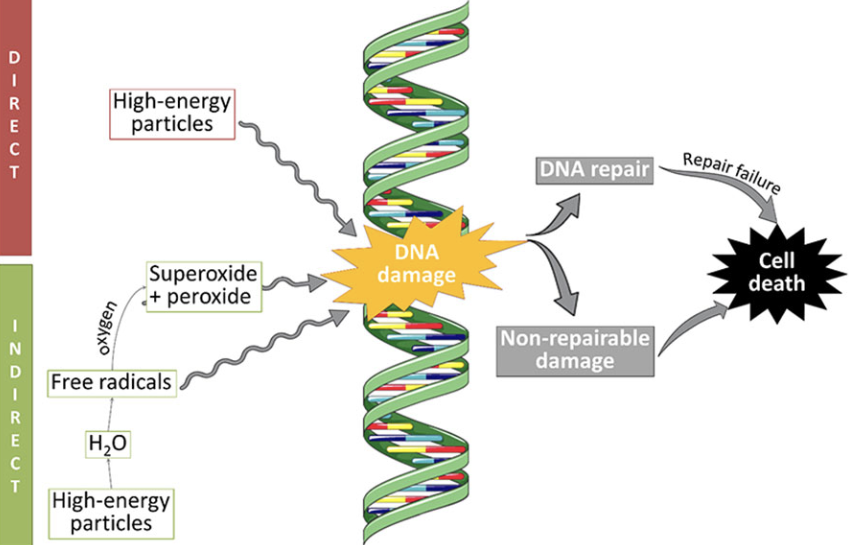
\includegraphics[width=\textwidth]{figure/radiation_DNA.png}
\textbackslash caption{[}Interaction of radiation and DNA{]}\{Interaction of radiation and DNA, adapted from Przystupski et al.(1), describes how high energy particles, which can be from radiation such as \(\alpha\), \(\beta\), and \(\gamma\), interacts with deoxyribonucleic acid.\}
\label{fig:radiationDNA}
\textbackslash end\{center\}
\textbackslash end\{figure\}

\hypertarget{refs}{}
\leavevmode\hypertarget{ref-przystupski_cytoprotective_2019}{}%
1. Przystupski D, Górska A, Rozborska P, Bartosik W, Michel O, Rossowska J, Szewczyk A, Drąg-Zalesińska M, Kasperkiewicz P, Górski J, Kulbacka J. 2019. The Cytoprotective Role of Antioxidants in Mammalian Cells Under Rapidly Varying UV Conditions During Stratospheric Balloon Campaign. Frontiers in Pharmacology 10.


% Index?

\end{document}
